\documentclass[a4paper,12pt]{report}

\usepackage{alltt, fancyvrb, url}
\usepackage{graphicx}
\usepackage[utf8]{inputenc}
\usepackage{float}
\usepackage{hyperref}
\usepackage[table]{xcolor}

% Questo commentalo se vuoi scrivere in inglese.
\usepackage[italian]{babel}
\usepackage[italian]{cleveref}
\usepackage[margin=1in]{geometry}
\usepackage{enumitem}

% Set the top margin to 0.5 inch
\setlength{\topmargin}{-0.3in}

\setlength{\parindent}{0pt}

\title{\textbf{Elaborato per il corso di\\"Basi di Dati"}
\\A.A. 2023/24}

\author{Gioele Bucci
\\ \texttt{gioele.bucci@studio.unibo.it}}
\date{\today}


\begin{document}

\maketitle

\tableofcontents

\chapter{Analisi dei requisiti}

Si vuole realizzare un sistema che consenta agli utenti di poter salvare ed analizzare delle partite al gioco da tavolo di strategia “RisiKo!”.
Ogni partita va memorizzata nel database, includendo i singoli turni: per ciascun turno deve essere possibile visualizzare sia lo stato di gioco che le azioni eseguite dal giocatore di turno.

\section{Intervista}

Un primo testo ottenuto dall’intervista è il seguente: \\ \\
Si vuole sviluppare un sistema che consenta agli utenti di memorizzare delle partite di Risiko, permettendo di visualizzarne lo stato nei vari turni. Per ciascun utente vengono salvati codice fiscale, nome, cognome e data di nascita. Un utente può partecipare come giocatore a più partite. \par
Ogni partita è caratterizzata da un codice identificativo, la data nella quale è avvenuta e il giocatore vincitore.
Ad ogni partita possono partecipare da 3 a 6 giocatori: per ciascuno si vuole memorizzare il relativo utente, un nickname, il colore dell’esercito scelto e l’obiettivo personale. \par
L’area di gioco è composta da un insieme di territori, identificati univocamente da un nome e per cui si memorizzano anche la lista di territori confinanti e il continente di appartenenza. \par
All’inizio di una partita ciascun giocatore riceve un numero predeterminato di carri armati, che dipende dal numero totale di giocatori partecipanti. Tutti i territori vengono poi distribuiti equamente tra i giocatori in modo casuale. In seguito, ogni giocatore posiziona tutte le sue armate sui propri territori, occupandone ciascuno con almeno un’unità. \par
Durante una partita, i giocatori si alternano ciclicamente in turni. \par
All’inizio di ogni turno avviene la fase di rinforzo, nella quale il giocatore di turno riceve una nuova armata per ogni tre territori in suo possesso. In aggiunta, il possesso di tutti i territori di un continente conferisce un bonus di armate aggiuntivo, che dipende dal continente conquistato. \par 
Le nuove armate ottenute vanno immediatamente posizionate dal giocatore di turno su uno o più territori che gli appartengono.
Ciascun turno all’interno di una partita è identificato da un numero e il nome del giocatore di turno. In aggiunta vanno registrati anche il numero di truppe presenti sui territori del giocatore dopo la fase di rinforzo, ed eventuali azioni compiute (uno spostamento e/o un attacco). \par
Per poter attaccare un territorio avversario, l’attaccante deve controllare un territorio ad esso adiacente. Per ciascun attacco vanno memorizzati l’attaccante, il difensore, il numero di truppe impiegate e perse da entrambe le parti e l’eventuale successo dell’attacco, che è considerato riuscito se tutte le truppe sul territorio avversario vengono eliminate. \par
Lo spostamento consiste nel muovere una parte delle proprie truppe da un territorio ad un altro ad esso adiacente (entrambi i territori devono appartenere allo stesso giocatore). Per ciascuno spostamento vanno memorizzati il territorio di partenza, quello di arrivo e il numero di truppe mobilitate. \par
I territori non possono mai essere lasciati vuoti e tale vincolo vale anche nel caso di attacchi e spostamenti: in entrambi i casi occorre che nel territorio di partenza rimanga almeno un’unità. Questo implica che in ogni momento di gioco ciascun territorio è controllato da un giocatore.

\section{Estrazione dei concetti principali}

\begin{itemize}
    \item \textbf{Utente}: persona fisica iscritta al sistema. Può partecipare a più partite come giocatore.
    \item \textbf{Giocatore}: colui che partecipa ad una partita. Ogni giocatore è associato ad un utente ed ha un colore, che rappresenta il suo esercito nel gioco, e un singolo obiettivo.
    \item \textbf{Obiettivo}: traguardo che un giocatore deve raggiungere per vincere la partita.
    \item \textbf{Territorio}: specifica regione di gioco, controllata da un solo giocatore alla volta. Ha dei territori confinanti e fa parte di un continente.
    \item \textbf{Continente}: insieme di più territori. Il possesso di un continente da parte di un giocatore gli conferisce un bonus di armate aggiuntive all’inizio del turno.
    \item \textbf{Armata}: unità militare controllata da un giocatore, utilizzata per conquistare e difendere territori. \\\textit{Sinonimi: unità, carro armato, truppa.}
    \item \textbf{Turno}: fase della partita comprendente una serie di azioni compiute da un singolo giocatore. I turni si susseguono ciclicamente tra i vari giocatori fino al termine della partita.
    \item \textbf{Attacco}: azione che un giocatore può svolgere nel proprio turno. Durante un attacco, il giocatore utilizza le armate presenti in un suo territorio per tentare di conquistare un territorio avversario adiacente.
    \item \textbf{Spostamento}: azione che un giocatore può svolgere nel proprio turno. Consiste nel muovere una parte di armate da un suo territorio ad uno adiacente, anch’esso di sua proprietà.

\end{itemize}

A seguito della lettura e comprensione dei requisiti, si procede redigendo un testo che ne riassuma tutti i concetti e in particolare ne estragga quelli principali eliminando le ambiguità sopra rilevate: \\ \\
Per ogni \textbf{\textit{utente}} del sistema vengono memorizzati codice fiscale, nome, cognome e data di nascita. \par
Ogni \textbf{\textit{partita}} è associata ad un codice identificativo, una data e un vincitore. \par
Ad una partita possono partecipare da 3 a 6 \textbf{\textit{giocatori}}: per ciascuno si memorizzano il relativo utente, un nickname, il colore dell'esercito scelto e l’obiettivo personale. \par
L’area di gioco è composta da vari \textbf{\textit{territori}}, identificati dal nome, e di cui si memorizzano anche la lista di territori confinanti e il continente di appartenenza. In ogni momento di gioco ciascun territorio è controllato da un solo giocatore.
Il numero di \textbf{\textit{armate}} conferite ad ogni giocatore all’inizio della partita viene stabilito in base al numero totale dei giocatori partecipanti. \par
Durante la partita, i giocatori si alternano ciclicamente in turni. Ogni \textbf{\textit{turno}} è identificato univocamente all’interno di una partita da un numero e il nome del giocatore di turno. Vanno inoltre memorizzati il numero di truppe presenti su ciascuno dei territori del giocatore, dopo la fase di rinforzo, ed eventuali azioni compiute. \par
Nella fase di rinforzo, che avviene all’inizio del turno, il giocatore riceve una nuova armata per ogni tre territori posseduti, oltre ad un eventuale bonus aggiuntivo per ogni \textbf{\textit{continente}} posseduto: tale bonus dipende dal continente. \par
Durante il proprio turno un giocatore può effettuare un attacco ad un territorio avversario e/o uno spostamento tra due territori adiacenti di sua proprietà. \par
Per ogni \textbf{\textit{attacco}} si registrano l'attaccante, il difensore, il numero di armate impiegate e perse da entrambe le parti e l'esito dell'attacco, che è considerato riuscito se tutte le armate sul territorio attaccato vengono eliminate. \par
Per ogni \textbf{\textit{spostamento}} si vogliono memorizzare il numero di armate mobilitate, il territorio di partenza e quello di arrivo.

\chapter{Progettazione concettuale}

Dall'analisi del dominio emerge che un \textbf{utente }è associato ad una persona fisica (l'identificatore è infatti il codice fiscale), mentre l'esistenza dell'entità \textbf{giocatore }è circoscritta alla specifica \textbf{partita} a cui partecipa. \par
La partecipazione all'associazione \textbf{vincitore}, che collega una partita ad un giocatore, è resa opzionale al fine di rendere possibile salvare anche partite non concluse. Inoltre, al giocatore devono essere associati l'\textbf{esercito} scelto e l'\textbf{obiettivo}, resi tramite delle entità. 

\begin{figure}[H]
\centering{}
\begin{center}
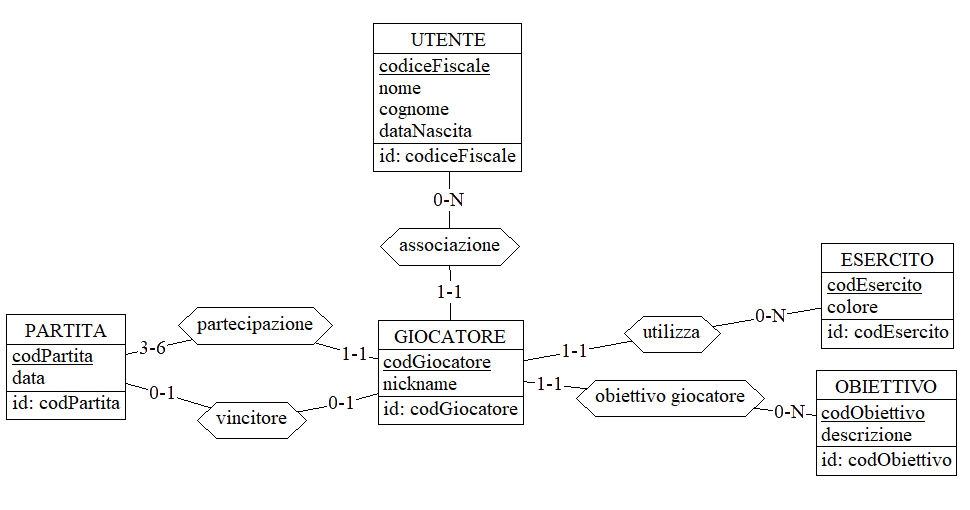
\includegraphics[width=\textwidth]{img/report/utente.png}
\end{center}
\emph{\caption{Schema E/R con le entità per la modellazione degli utenti e giocatori}}
\label{img:utente}
\end{figure}

Una partita è suddivisa in più turni: ciascun \textbf{turno} è identificato univocamente all'interno della partita mediante un numero e il nome del giocatore di turno. Pertanto, si utilizzano come identificatori il numero del turno, il giocatore (tramite l'associazione \textbf{effettuazione turno}) e la partita (tramite l'associazione \textbf{suddivisione}).   \par
Per memorizzare i \textbf{territori} posseduti e il numero di \textbf{armate} presenti su di essi, si utilizza l'associazione \textbf{controllo territorio}.

\begin{figure}[H]
\centering{}
\begin{center}
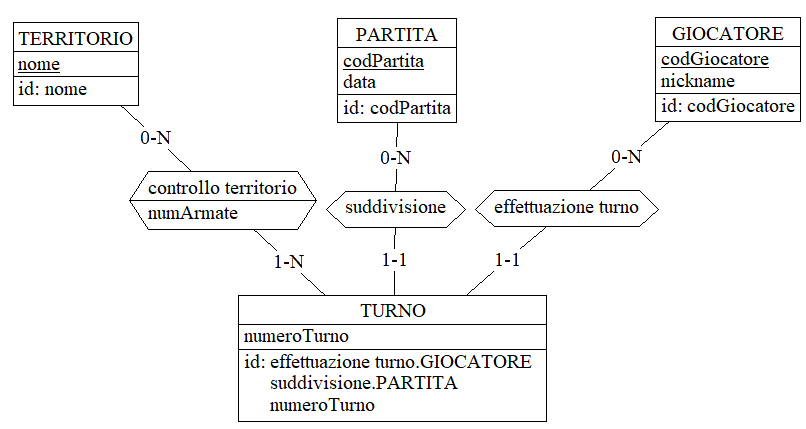
\includegraphics[width=\textwidth]{img/report/turno_par.png}
\end{center}
\emph{\caption{Schema E/R con una modellazione parziale dei turni}}
\label{img:turno_par}
\end{figure}
In ogni turno si possono effettuare un \textbf{attacco} e uno \textbf{spostamento}, entrambi resi tramite entità e identificati da un codice univoco. \par
L’esito di un attacco è dato dalla flag booleana \textit{vittoria}, mentre il territorio \textbf{attaccante} e quello \textbf{difensore} sono resi tramite associazioni. \par
Ci sono dei vincoli inespressi per cui il territorio attaccante e quello difensore devono essere diversi, confinanti e appartenenti a giocatori differenti. \par
Gli spostamenti sono modellati in maniera analoga agli attacchi e nell’entità si memorizza il numero di armate mobilitate. Il territorio di partenza e quello di arrivo sono resi, rispettivamente, dalle associazioni \textbf{da}, \textbf{a}. \par
Anche in questo caso ci sono dei vincoli inespressi per cui il territorio di partenza e quello di arrivo devono essere diversi, confinanti e appartenenti allo stesso giocatore. 

\begin{figure}[H]
\centering{}
\begin{center}
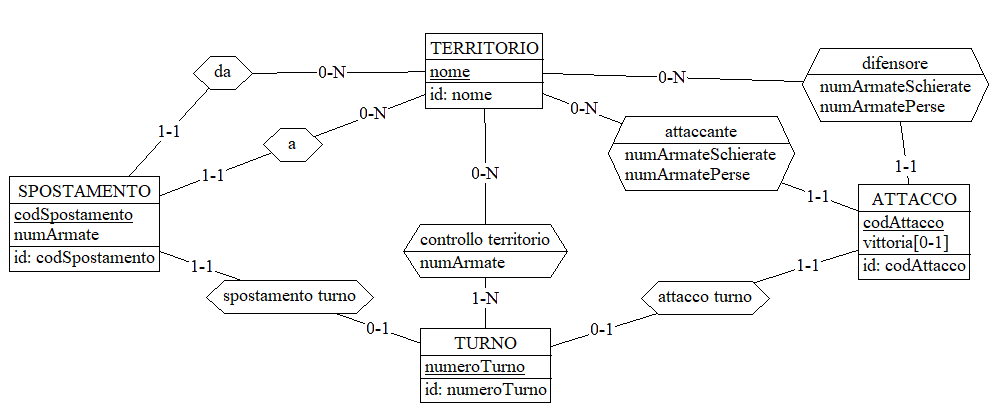
\includegraphics[width=\textwidth]{img/report/turno.png}
\end{center}
\emph{\caption{Schema E/R con la modellazione completa dei turni}}
\label{img:turno_par}
\end{figure}

Ogni territorio confina con almeno un’altro territorio (associazione ad anello simmetrica \textbf{confinante}) e fa parte di un \textbf{continente}, modellato tramite un’entità e identificato univocamente dal nome. \par
Infine, per memorizzare il numero di armate iniziali da assegnare in base al numero totale di giocatori, è stata aggiunta un’entità \textbf{armate iniziali}. \par
Di seguito lo schema finale:
\begin{figure}[H]
\centering{}
\begin{center}
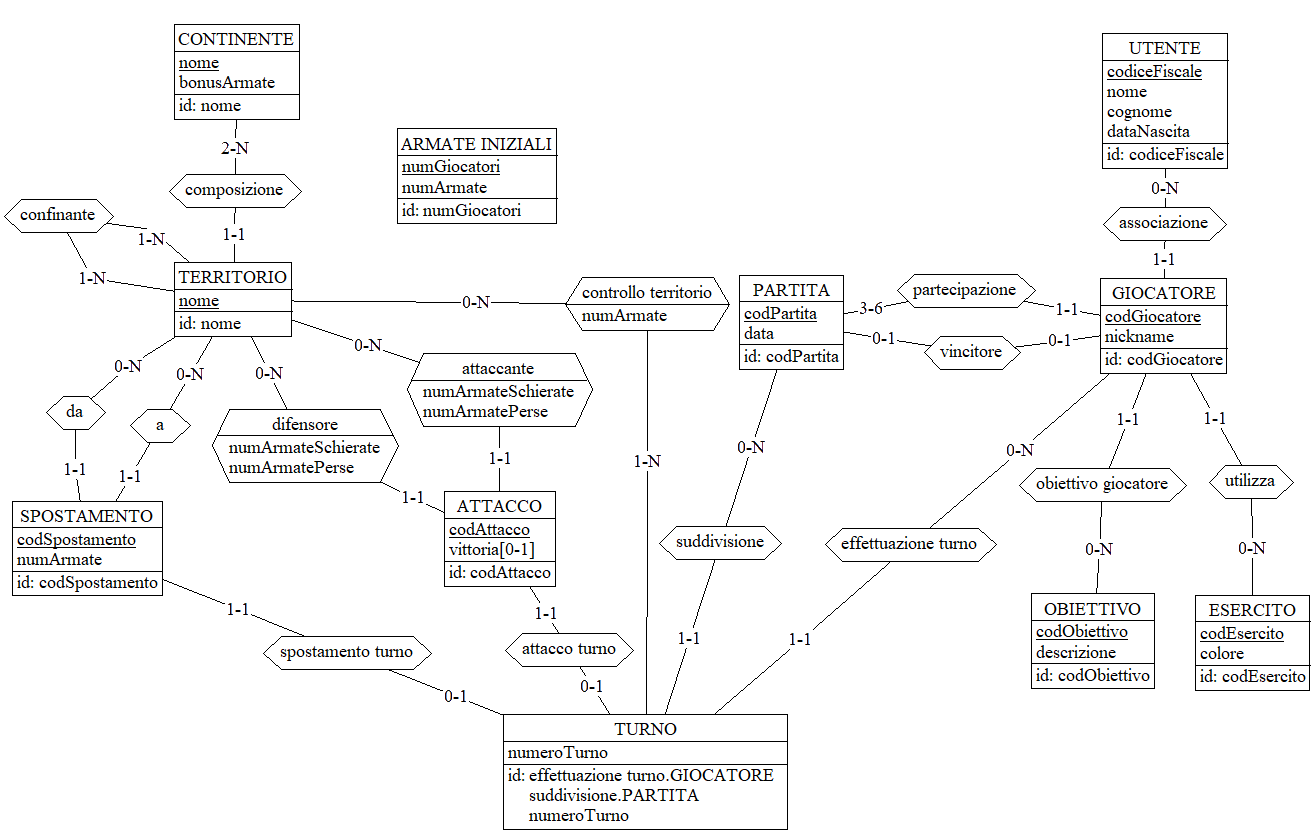
\includegraphics[width=\textwidth]{img/report/finale.png}
\end{center}
\label{img:turno_par}
\end{figure}

\chapter{Progettazione logica}
\section{Stima del volume dei dati}

\begin{table}[H]
    \centering
    \begin{tabular}{|c|c|c|}
        \hline
        \rowcolor{lime!50} 
        \textbf{Concetto}& \textbf{Costrutto}& \textbf{Volume}\\ \hline
        Continente & E & 6 \\ \hline 
        Composizione & R & 42 \\ \hline 
        Territorio & E & 42 \\ \hline 
        Confinante & R & 168\\ \hline 
        Armate Iniziali & E & 4 \\ \hline
        Obiettivo & E & 14 \\ \hline 
        Esercito & E & 6 \\ \hline 
        Utente & E & 10.000 \\ \hline
        Giocatore & E & 450.000 \\ \hline 
        Associazione & R & 450.000 \\ \hline 
        Partita & E & 100.000 \\ \hline 
        Vincitore & R & 95.000 \\ \hline 
        Partecipazione & R & 450.000 \\ \hline 
        Utilizza & R & 450.000 \\ \hline 
        Obiettivo Giocatore & R & 450.000 \\ \hline 
        Turno & E & 7.200.000 \\ \hline
        Effettuazione Turno & R & 7.200.000 \\ \hline
        Suddivisione & R & 7.200.000 \\ \hline
        Controllo Territorio & R & 67.200.000\\ \hline
        Spostamento & E & 6.300.000 \\ \hline 
        Spostamento Turno & R & 6.300.000 \\ \hline 
        Da & R & 6.300.000 \\ \hline 
        A & R & 6.300.000 \\ \hline 
        Attacco & E & 5.400.000 \\ \hline 
        Attacco Turno & R & 5.400.000 \\ \hline 
        Attaccante & R & 5.400.000 \\ \hline 
        Difensore & R & 5.400.000 \\ \hline 
    \end{tabular}
\end{table}

\section{Descrizione delle operazioni principali}

Segue una lista delle operazioni da effettuare e la relativa frequenza:

\begin{table}[htbp]
    \begin{tabular}{lll}
        \rowcolor{lime!50} 
        \textbf{N.} & \textbf{Operazione} & \textbf{Freq.} \\
        1 & Registrare un nuovo utente & 2/g \\ 
        2 & Registrare una nuova partita & 10/g \\ 
        3 & Determinare il numero di armate iniziali da assegnare ai giocatori & 10/g \\ 
        4 & Registrare un nuovo turno all'interno di una partita & 160/g \\
        5 & Mostrare il giocatore a cui appartiene un territorio in un certo turno & 500/g \\ 
        6 & Registrare un attacco & 120/g \\ 
        7 & Registrare uno spostamento & 140/g \\ 
        8 & Determinare le armate da assegnare ad un giocatore nella fase di rinforzo & 160/g \\ 
        9 & Mostrare la classifica dei giocatori, in base al numero di territori posseduti & 160/g \\
        10 & Registrare una vittoria & 9/g \\
        11 & Mostrare la classifica globale degli utenti, in base al numero di vittorie & 1/set \\
    \end{tabular}
\end{table}

\section{Schemi di navigazione e tabelle degli accessi}

Si riportano di seguito le tabelle degli accessi per le operazioni sopra descritte. \par
Si noti che, al fine del calcolo dei costi, gli accessi in scrittura sono considerati di peso doppio rispetto a quelli in lettura.

\subsubsection{OP 1 - Registrare un nuovo utente}

\begin{table}[htbp]
    \begin{tabular}{cccc}
        \rowcolor{lime!50} 
        \textbf{Concetto}& \textbf{Costrutto}& \textbf{Accessi} & \textbf{Tipo} \\ \hline 
        Utente & E & 1 & S \\ \hline
        \rowcolor{lime!50} 
        \multicolumn{4}{c}{\textbf{Totale:} 2L * 2 $\rightarrow$ 4 al giorno } \\ 
    \end{tabular}
\end{table}

\subsubsection{OP 2 - Registrare una nuova partita}

Dato che un'istanza di giocatore è valida solo all'interno della partita alla quale partecipa, al momento della creazione
di una nuova partita vengono creati anche i relativi giocatori, che in media sono 4.5, assegnandovi un esercito ed un obiettivo casuale.

\begin{table}[htbp]
    \begin{tabular}{cccc}
        \rowcolor{lime!50} 
        \textbf{Concetto}& \textbf{Costrutto}& \textbf{Accessi} & \textbf{Tipo}\\ \hline
        Partita & E & 1 & S \\ \hline
        Giocatore & E & 4.5 & S \\ \hline
        Associazione & R & 4.5 & S \\ \hline
        Obiettivo Giocatore & R & 4.5 & S \\ \hline
        Utilizza & R & 4.5 & S \\ \hline
        Partecipazione & R & 4.5 & S \\ \hline
        \rowcolor{lime!50} 
        \multicolumn{4}{c}{\textbf{Totale:} 23.5S * 10 $\rightarrow$ 470 al giorno } \\ 
    \end{tabular}
\end{table}

\subsubsection{OP 3 - Determinare il numero di armate iniziali da assegnare ai giocatori}

Questa operazione viene svolta all'inizio di ogni partita (si suppone che tale partita sia già stata creata). \par
Occorre contare i giocatori partecipanti e leggere il corrispondente numero di armate iniziali.

\begin{table}[htbp]
    \begin{tabular}{cccc}
        \rowcolor{lime!50} 
        \textbf{Concetto}& \textbf{Costrutto}& \textbf{Accessi} & \textbf{Tipo}\\ \hline
        Partecipazione & A & 4.5 & L \\ \hline
        Armate Iniziali & E & 1 & L \\ \hline
        \rowcolor{lime!50} 
        \multicolumn{4}{c}{\textbf{Totale:} 5.5L * 10 $\rightarrow$ 55 al giorno } \\ 
    \end{tabular}
\end{table}


\subsubsection{OP 4 - Registrare un nuovo turno}

È necessario, in particolare, memorizzare i territori posseduti ad inizio turno, mediamente 9.33 (42 territori divisi tra 4.5 giocatori).

\begin{table}[htbp]
    \begin{tabular}{cccc}
        \rowcolor{lime!50} 
        \textbf{Concetto}& \textbf{Costrutto}& \textbf{Accessi} & \textbf{Tipo}\\ \hline
        Turno & E & 1 & S \\ \hline
        Suddivisione & R & 1 & S \\ \hline
        Effettuazione Turno & R & 1 & S \\ \hline
        Controllo Territorio & R & 9.33 & S \\ \hline
        \rowcolor{lime!50} 
        \multicolumn{4}{c}{\textbf{Totale:} 12.33S * 160 $\rightarrow$ 3946 al giorno } \\ 
    \end{tabular}
\end{table}

\subsubsection{OP 5 - Mostrare il giocatore a cui appartiene un territorio} 

Per trovare il giocatore al quale appartiene un certo territorio al turno numero $n$, occorre controllare l'$n$-esimo turno di tutti i giocatori.  \par
Ci sono in media 4.5 giocatori/partita e la somma dei territori da essi controllati in un qualsiasi turno $n$ deve corrispondere al numero totale di territori presenti, ovvero 42.  \par
Nel caso peggiore occorre perciò controllare tutte le 42 istanze di "\textit{Controllo Territorio}", distribuite nei 4,5 turni. \par

\begin{table}[H]
    \begin{tabular}{cccc}
        \rowcolor{lime!50} 
        \textbf{Concetto}& \textbf{Costrutto}& \textbf{Accessi} & \textbf{Tipo} \\ \hline
        Turno & E & 4.5 & L \\ \hline
        Controllo Territorio & R & 42 & L \\ \hline
        \rowcolor{lime!50} 
        \multicolumn{4}{c}{\textbf{Totale:} 46.5L * 500 $\rightarrow$ 23250 al giorno } \\ 
    \end{tabular}
\end{table}


\subsubsection{OP 6 - Registrare un attacco}

Si assume che il turno sia già stato creato. \par
Per portare a termine l'operazione è necessario verificare che i due territori, attaccante e difensore, siano:
\begin{itemize}
    \item \textbf{diversi}: occorre la lettura dei 2 territori.
    \item \textbf{confinanti}: è sufficiente verificare che uno dei due territori confini con l'altro, poichè la relazione è simmetrica (se A confina con B allora B confina con A). Ci sono 42 territori e 168 confini, quindi in media andranno eseguite 4 letture.
    \item \textbf{appartenenti a giocatori differenti}: per il giocatore di turno basta leggere i territori controllati, mentre per il difensore tale informazione va ricavata in maniera analoga alla query precedente, controllando per tutti i giocatori \textit{meno l'attaccante}.
\end{itemize}

Per rendere più agevole la comprensione della tabella degli accessi si evidenziano i costi extra relativi ai controlli sopra indicati.
\begin{table}[htbp]
    \begin{tabular}{cccc}
        \rowcolor{lime!50} 
        \textbf{Concetto}& \textbf{Costrutto}& \textbf{Accessi} & \textbf{Tipo}\\ \hline
        Attacco Turno & R & 1 & S \\ \hline
        Attacco & E & 1 & S \\ \hline
        Attaccante & R & 1 & S \\ \hline
        Difensore & R & 1 & S \\ \hline
        % CHECKS %
        \rowcolor{orange!20} 
        Territorio & E & 2 & L \\ \hline
        \rowcolor{orange!20} 
        Confinante & R & 4 & L \\ \hline
        \rowcolor{orange!20} 
        Controllo Territorio & R & 9.33 & L \\ \hline
        \rowcolor{orange!20} 
        Turno & E & 3.5 & L \\ \hline
        \rowcolor{orange!20} 
        Controllo Territorio & R & 32.67 & L \\ \hline
        \rowcolor{lime!50} 
        \multicolumn{4}{c}{\textbf{Totale:} (51.5L + 4S) * 120 $\rightarrow$ 7140 al giorno } \\ 
        \end{tabular}
\end{table}

\subsubsection{OP 7 - Registrare uno spostamento}

Si assume che il turno sia già stato creato. \par
Per portare a termine l'operazione è necessario verificare che i due territori siano diversi, confinanti e appartenenti allo stesso giocatore. I primi due controlli sono analoghi a queli effettuati nel caso dell'attacco, mentre per controllare se i territori appartengono allo stesso giocatore è sufficiente leggerne i territori controllati.
\begin{table}[htbp]
    \begin{tabular}{cccc}
        \rowcolor{lime!50} 
        \textbf{Concetto}& \textbf{Costrutto}& \textbf{Accessi} & \textbf{Tipo}\\ \hline
        Spostamento Turno & R & 1 & S \\ \hline
        Spostamento & E & 1 & S \\ \hline
        Da & R & 1 & S \\ \hline
        A & R & 1 & S \\ \hline
        % CHECKS %
        \rowcolor{orange!30} 
        Territorio & E & 2 & L \\ \hline
        \rowcolor{orange!30} 
        Confinante & R & 4 & L \\ \hline
        \rowcolor{orange!30} 
        Controllo Territorio & R & 9.33 & L \\ \hline
        \rowcolor{lime!50} 
        \multicolumn{4}{c}{\textbf{Totale:} (15.33L + 4S) * 140 $\rightarrow$ 3266 al giorno } \\ 
    \end{tabular}
\end{table}

\subsubsection{OP 8 - Determinare le armate da assegnare ad un giocatore nella fase di rinforzo} 

Tale operazione viene eseguita nel contesto di un turno. Occorre leggere tutti i territori controllati dal giocatore e verificare se possiede uno o più continenti (6 in totale).

\begin{table}[H]
    \begin{tabular}{cccc}
        \rowcolor{lime!50} 
        \textbf{Concetto}& \textbf{Costrutto}& \textbf{Accessi} & \textbf{Tipo}\\ \hline
        Controllo Territorio & R & 9.33 & L \\ \hline
        Continente & E & 6 & L \\ \hline
        \rowcolor{lime!50} 
        \multicolumn{4}{c}{\textbf{Totale:} 10.33L * 160 $\rightarrow$ 2453 al giorno } \\ 
    \end{tabular}
\end{table}

\subsubsection{OP 9 - Mostrare la classifica dei giocatori, in base al numero di territori posseduti}

Tale operazione viene eseguita nel contesto di un certo turno di numero $n$. \par
Per ciascun giocatore è necessario contare i relativi territori posseduti al turno $n$-esimo.

\begin{table}[H]
    \begin{tabular}{cccc}
        \rowcolor{lime!50} 
        \textbf{Concetto}& \textbf{Costrutto}& \textbf{Accessi} & \textbf{Tipo}\\ \hline
        Turno & E & 4.5 & L \\ \hline
        Controllo Territorio & R & 42 & L \\ \hline
        \rowcolor{lime!50} 
        \multicolumn{4}{c}{\textbf{Totale:} 46.5L * 160 $\rightarrow$ 7440 al giorno } \\ 
    \end{tabular}
\end{table}

\subsubsection{OP 10 - Registrare una vittoria}

\begin{table}[H]
    \begin{tabular}{cccc}
        \rowcolor{lime!50} 
        \textbf{Concetto}& \textbf{Costrutto}& \textbf{Accessi} & \textbf{Tipo}\\ \hline
        Vincitore & R & 1 & S \\ \hline
        \rowcolor{lime!50} 
        \multicolumn{4}{c}{\textbf{Totale:} 1S * 9 $\rightarrow$ 18 al giorno } \\ 
    \end{tabular}
\end{table}

\subsubsection{OP 11 - Mostrare la classifica globale degli utenti, in base al numero di vittorie}        

Leggendo tutte le tuple da "\textit{Vincitore}" è possibile risalire ai giocatori e successivamente ai relativi utenti. 

\begin{table}[H]
    \begin{tabular}{cccc}
        \rowcolor{lime!50} 
        \textbf{Concetto}& \textbf{Costrutto}& \textbf{Accessi} & \textbf{Tipo}\\ \hline
        Vincitore & R & 95.000 & L \\ \hline
        Giocatore & E & 95.000 & L \\ \hline
        Utente & E & 95.000 & L \\ \hline
        \rowcolor{lime!50} 
        \multicolumn{4}{c}{\textbf{Totale:} 285000L $\rightarrow$ 285000 a settimana } \\ 
    \end{tabular}
\end{table}

\pagebreak

\section{Raffinamento dello schema}

Nello schema E/R sono state eliminate le seguenti relazioni:
\begin{itemize}
    \setlength\itemsep{1pt}
    \item Associazione, importando codiceFiscale (rinominato in codUtente) in Giocatore
    \item Obiettivo Giocatore, importando codObiettivo in Giocatore
    \item Utilizza, importando codEsercito in Giocatore
    \item Partecipazione, importando codPartita in Giocatore
    \item Effettuazione Turno, importando codGiocatore in Turno
    \item Suddivisione, importando codPartita in Turno
    \item Attacco Turno, importando codAttacco in Turno e rendendolo opzionale
    \item Spostamento Turno, importando codSpostamento in Turno e rendendolo opzionale
    \item Da, importando nome (rinominato in territorioPartenza) in Spostamento
    \item A, importando nome (rinominato in territorioArrivo) in Spostamento
    \item Composizione, importando nome (rinominato in continente) in Territorio
    \item Vincitore, reificata importando codPartita da Partita e codGiocatore da Giocatore
    \item Controllo Territorio, reificata importando numeroTurno, codPartita e codGiocatore da Turno e nome da Territorio
    \item Attaccante, esportandone gli attributi (armateSchierate e armatePerse) in Attacco 
    \item Difensore, esportandone gli attributi (difArmateSchierate e difArmatePerse) in Attacco 
    \item Confinante, reificata importando nome da Territorio (rinominati in terrA e terrB)
\end{itemize}

\pagebreak

\section{Analisi delle ridondanze}

\subsubsection{OP 9 - Mostrare la classifica dei giocatori, in base al numero di territori controllati}

È stata inserita una ridondanza aggiungendo in Turno l'attributo ridondante \textit{territoriControllati}.
Come si può vedere dalla tabella sottostante, tale ridondanza agevola notevolmente l'operazione di conteggio dei territori:

\begin{table}[H]
    \begin{tabular}{cccc}
        \rowcolor{lime!50} 
        \textbf{Concetto}& \textbf{Costrutto}& \textbf{Accessi} & \textbf{Tipo}\\ \hline
        Turno & E & 4.5 & L \\ \hline
        \rowcolor{lime!50} 
        \multicolumn{4}{c}{\textbf{Totale:} 4.5L * 160 $\rightarrow$ 720 al giorno } \\ 
    \end{tabular}
\end{table}

Senza ridondanza:

\begin{table}[H]
    \begin{tabular}{cccc}
        \rowcolor{yellow!50} 
        \textbf{Concetto}& \textbf{Costrutto}& \textbf{Accessi} & \textbf{Tipo}\\ \hline
        Turno & E & 4.5 & L \\ \hline
        Controllo Territorio & R & 42 & L \\ \hline
        \rowcolor{yellow!50} 
        \multicolumn{4}{c}{\textbf{Totale:} 46.5L * 160 $\rightarrow$ 7440 al giorno } \\ 
    \end{tabular}
\end{table}

\subsubsection{OP 11 - Mostrare la classifica globale degli utenti, in base al numero di vittorie}        

Introducendo l'attributo ridondante "\textit{vittorie}" in Utente è possibile redigere la classifica effettuando molte meno letture, poichè è suficiente leggere tutti gli utenti. \par

\begin{table}[H]
    \begin{tabular}{cccc}
        \rowcolor{lime!50} 
        \textbf{Concetto}& \textbf{Costrutto}& \textbf{Accessi} & \textbf{Tipo}\\ \hline
        Utente & E & 10000 & L \\ \hline
        \rowcolor{lime!50} 
        \multicolumn{4}{c}{\textbf{Totale:} 10000L $\rightarrow$ 10000 a settimana } \\ 
    \end{tabular}
\end{table}

Senza ridondanza:

\begin{table}[H]
    \begin{tabular}{cccc}
        \rowcolor{yellow!50} 
        \textbf{Concetto}& \textbf{Costrutto}& \textbf{Accessi} & \textbf{Tipo}\\ \hline
        Vincitore & R & 95.000 & L \\ \hline
        Giocatore & E & 95.000 & L \\ \hline
        Utente & E & 95.000 & L \\ \hline
        \rowcolor{yellow!50} 
        \multicolumn{4}{c}{\textbf{Totale:} 285000L $\rightarrow$ 285000 a settimana } \\ 
    \end{tabular}
\end{table}

Per completezza si sottolinea che l'introduzione di un attributo ridondante comporta anche un aumento nel costo dell'operazione 10 (registrazione di una vittoria), che passa da 18/g a 45/g, come mostrato nella tabella sottostante. \par 

\begin{table}[H]
    \begin{tabular}{cccc}
        \rowcolor{lime!50} 
        \textbf{Concetto}& \textbf{Costrutto}& \textbf{Accessi} & \textbf{Tipo}\\ \hline
        Vincitore & R & 1 & S \\ \hline
        Utente & R & 1 & L \\ \hline
        Utente & R & 1 & S \\ \hline
        \rowcolor{lime!50} 
        \multicolumn{4}{c}{\textbf{Totale:} (1L + 2S) * 9 $\rightarrow$ 45 al giorno } \\ 
    \end{tabular}
\end{table}

\pagebreak

Calcolo dei costi senza ridondanza:

\begin{itemize}
    \item OP 10: 285000 a settimana
    \item OP 11: 18 * 7 = 126 a settimana
\end{itemize}

\textbf{Totale}: 285126 a settimana. \\ \\
Con ridondanza:

\begin{itemize}
    \item OP 10: 10000 a settimana
    \item OP 11: 45 * 7 = 315 a settimana
\end{itemize}

\textbf{Totale}: 10315 a settimana. \par
Dopo aver analizzato la variazione nei costi delle due operazioni sull'arco di una settimana, emerge che conviene mantenere la ridondanza.  

\section{Traduzione di entità e associazioni in relazioni}

\begin{description}
    \item \textbf{UTENTI} (\underline{codiceFiscale}, nome, cognome, dataNascita, vittorie) \par
    \item \textbf{PARTITE} (\underline{codPartita}, data) \par
    \item \textbf{OBIETTIVI} (\underline{codObiettivo}, descrizione) \par
    \item \textbf{ESERCITI} (\underline{codEsercito}, colore) \par
    \item \textbf{GIOCATORI} (\underline{codGiocatore}, nickname, codUtente: UTENTI, codPartita: PARTITE, codObiettivo: OBIETTIVI, codEsercito: ESERCITI) \par
    \item \textbf{VINCITORI} (\underline{codPartita}: PARTITE, codGiocatore: GIOCATORI) \par
    \item \textbf{ARMATE\_INIZIALI} (\underline{numGiocatori}, numArmate) \par
    \item \textbf{TURNI} ((\underline{numeroTurno}, \underline{codParita}: PARTITE, \underline{codGiocatore}: GIOCATORI), territoriControllati, codSpostamento*: SPOSTAMENTI, codAttacco*: ATTACCHI) \par
    \item \textbf{ATTACCHI} (\underline{codAttacco}, vittoria*, armateSchierate, armatePerse, difArmateSchierate, difArmatePerse, attaccante: TERRITORI, difensore: TERRITORI) \par
    \item \textbf{SPOSTAMENTI} (\underline{codSpostamento}, numArmate, territorioPartenza: TERRITORI, territorioArrivo: TERRITORI) \par
    \item \textbf{CONTINENTI} (\underline{nome}, bonusArmate) \par
    \item \textbf{TERRITORI} (\underline{nome}, continente: CONTINENTI) \par
    \item \textbf{CONFINI} ((\underline{terrA}: TERRITORI, \underline{terrB}: TERRITORI)) \par
    \item \textbf{CONTROLLI\_TERRITORIO} (((\underline{numeroTurno}, \underline{codParita}, \underline{codGiocatore}): TURNI, \underline{territorio}: TERRITORI), numArmate) \par
\end{description}

\section{Schema relazione finale}
\section{Traduzione delle operazioni in query SQL}
\chapter{Progettazione dell'applicazione}
\section{Descrizione dell'architettura dell'applicazione realizzata}

\end{document}
